% Chapter X

\chapter{One Way Quantum Computation} % Chapter title

\label{ch:measurement} % For referencing the chapter elsewhere, use \autoref{ch:name} 

 In order to demonstrate how numerical simulation of one way quantum computation might be achieved, the first step is to examine the operation of the one way quantum computation. This involves examination of how cluster states can be formed as well as the function performed by measurement so that these procedures can be included in the simulation. In this regard, the procedures for functionality are detailed here so they might be compared to the program in later section to verify correct functionality.

%----------------------------------------------------------------------------------------

\section{Hamiltonian on interacting particles}
Following the work in 'Persistant Entanglement In Arrays of Interacting Particles', the Hamiltonian for a d-dimensional lattice at sites $a \in \mathbb{Z}^{d}$ interacting through short range interaction is \citep{briegel_persistent_2000}:

\begin{equation}
\label{eq:h_int}
\hat{H} _{int} = \hbar g(t) \sum\limits_{a, a'} f(a - a') \frac{1 - \sigma^{a}_{z}}{2} \frac{1 - \sigma^{a'}_{z}}{2}
\end{equation}

where:
\begin{align*}
f(a - a') &- \mbox{interaction range} \\
g(t) &- \mbox{time dependence of interaction} \\
\sigma_{z} &- \mbox{pauli-z operation}
\end{align*}

From the time dependent Schr\"{o}dinger equation we extract the time evolution of a wavefunction:

\begin{equation}
i\hbar \frac{\partial}{\partial t} \ket{\Psi} = \hat{H} \ket{\Psi}
\end{equation}

\begin{equation}
\ket{\Psi (t)} = e^{- \frac{i \hat{H} t}{\hbar}} \ket{\Psi (0)}
\end{equation}

From which we extract the time dependence operator:

\begin{equation}
\label{eq:td_op}
\hat{U} (t) = e^{- \frac{i \hat{H} t}{\hbar}}
\end{equation}

Substituting the interaction Hamiltonian \eqref{eq:h_int} into the time dependence operator\eqref{eq:td_op} gives:

\begin{equation}
\label{eq:td_op_h}
\hat{U} (t) = exp\left(-i g(t) t \sum\limits_{a, a'} f(a - a') \frac{1 - \sigma^{a}_{z}}{2} \frac{1 - \sigma^{a'}_{z}}{2}\right)
\end{equation}

Considering a one-dimensional chain of N-qubits with only next neighbour interactions the interaction range can be expressed as:

\begin{equation}
f(a - a') = \delta _{a + 1, a}
\end{equation}

Which will prevent qubits interacting with themselves and allow nearest neighbour interactions. Now we introduce a term $\phi$ which represents the integration of the time dependence of interaction such that:

\begin{equation}
\phi = \int g(t) \, dt = C g(t) t + D
\end{equation}

Where C and D are constants. Therefore the time evolution operator becomes

\begin{equation}
\label{eq:td_op_phi}
\hat{U} (t) = exp\left(-i \phi \sum\limits_{a} \frac{1 - \sigma^{a}_{z}}{2} \frac{1 - \sigma^{a + 1}_{z}}{2}\right)
\end{equation}

 

%------------------------------------------------

\section{Two qubit cluster state}

We can further refine this operator for the interaction between two qubits through the use of Euler's relation for operators:

\begin{equation}
\label{eq:euler}
e^{i  \theta \hat{A}} = \cos(\theta) \hat{\mathbb{1}} + i \sin (\theta) \hat{A}
\end{equation}

Now,we can expand the equation \eqref{eq:td_op_phi} as there are only two qubits to give:

\begin{equation}
\label{eq:td_op_phi_exp}
\hat{U} (t) = exp\left(-\frac{i \phi}{4} \left(\mathbb{1} \otimes \mathbb{1} - \mathbb{1} \otimes \sigma_{z} - \sigma_{z} \otimes \mathbb{1} + \sigma_{z} \otimes \sigma_{z} \right)\right)
\end{equation}

Typically we would need to apply the Baker-Campbell-Hausdorff formula to convert these terms into something more manageable, however the operators $\mathbb{1}$ and $\sigma_{z}$ are commutative, as are their tensor products, so all but the first two terms of the Baker-Campbell-Hausdorff expansion can be neglected leaving:

\begin{equation}
\hat{U} (t) = exp(-\frac{i \phi}{4} \mathbb{1} \otimes \mathbb{1})
exp(\frac{i \phi}{4} \sigma_{z} \otimes \mathbb{1})
exp(\frac{i \phi}{4} \sigma_{z} \otimes \mathbb{1}) 
exp(-\frac{i \phi}{4} \sigma_{z} \otimes \sigma_{z})
\end{equation}

Applying equation \eqref{eq:euler}:

\begin{multline}
\hat{U} (t) = exp(-\frac{i \phi \mathbb{1}}{4}) \\
\left(\cos(\frac{i \phi}{4}) \mathbb{1} \otimes \mathbb{1}
+ i \sin (\frac{i \phi}{4}) \mathbb{1} \otimes \sigma_{z}\right) \\
\left(\cos(\frac{i \phi}{4}) \mathbb{1} \otimes \mathbb{1}
+ i \sin (\frac{i \phi}{4}) \sigma_{z} \otimes \mathbb{1}\right) \\
\left(\cos(\frac{-i \phi}{4}) \mathbb{1} \otimes \mathbb{1}
+ i \sin (\frac{-i \phi}{4}) \sigma_{z} \otimes \sigma_{z}\right) \\
\end{multline}

In the case of $\phi = \pi$ this becomes:

\begin{multline}
\hat{U} (t) = \frac{1}{2 \sqrt{2}}exp(-\frac{i \pi}{4}) \mathbb{1} \\
\left( \mathbb{1} \otimes \mathbb{1}
+ i \mathbb{1} \otimes \sigma_{z}\right) \\
\left( \mathbb{1} \otimes \mathbb{1}
+ i \sigma_{z} \otimes \mathbb{1}\right) \\
\left( \mathbb{1} \otimes \mathbb{1}
- i \sigma_{z} \otimes \sigma_{z}\right) \\
\end{multline}

Now, expanding brackets and simplifying in two steps:

\begin{multline*}
\hat{U} (t) = \frac{1}{2 \sqrt{2}}exp(-\frac{i \pi}{4}) \mathbb{1} \\
\left( \mathbb{1} \otimes \mathbb{1}
- \sigma_{z} \otimes \sigma_{z}
+ i \mathbb{1} \otimes \sigma_{z}
+ i \sigma_{z} \otimes \mathbb{1} \right) \\
\left( \mathbb{1} \otimes \mathbb{1}
- i \sigma_{z} \otimes \sigma_{z}\right) \\ \\
 = \frac{1}{2 \sqrt{2}}exp(-\frac{i \pi}{4}) \\
( \mathbb{1} \otimes \mathbb{1}
- \sigma_{z} \otimes \sigma_{z}
+ i \mathbb{1} \otimes \sigma_{z}
+ i \sigma_{z} \otimes \mathbb{1} \\
+ i \mathbb{1} \otimes \mathbb{1}
- i \sigma_{z} \otimes \mathbb{z}
+ \mathbb{1} \otimes \sigma_{z}
+ \sigma_{z} \otimes \mathbb{1} ) \\
\end{multline*}

Factorising real and imaginary terms:

\begin{multline}
\label{eq:u_last_simp}
\hat{U} (t) = \frac{1}{2}
exp(-\frac{i \pi}{4}) 
\frac{1 + i}{\sqrt{2}} \\
\left( \mathbb{1} \otimes \mathbb{1}
- \sigma_{z} \otimes \sigma_{z}
+ \mathbb{1} \otimes \sigma_{z}
+ \sigma_{z} \otimes \mathbb{1}\right) \\
\end{multline}

As $exp(-\frac{i \pi}{4}) = \frac{1 - i}{\sqrt{2}}$ equation \eqref{eq:u_last_simp} simplifies to:

\begin{multline}
\label{eq:u_final}
\hat{U} (t) = \frac{1}{2}
\left( \mathbb{1} \otimes \mathbb{1}
+ \mathbb{1} \otimes \sigma_{z}
+ \sigma_{z} \otimes \mathbb{1}
- \sigma_{z} \otimes \sigma_{z}\right) \\
\end{multline}

If this operator is applied to two qubits in the $\ket{+ +}$ state, for example, we get:

\begin{multline}
\label{eq:2qubit_example}
\hat{U} (t) \ket{+ +} = \frac{1}{2}
(\ket{++} + \ket{+-} + \ket{-+} - \ket{--}) \\ \\
= \frac{1}{\sqrt{2}} (\ket{+ 0} + \ket{- 1}) \\
\end{multline}

%------------------------------------------------

\section{Three qubit cluster state}

By using the same method used in the previous section, we can also obtain a the time evolution operator for a chain of three qubits only interacting with their nearest neighbour. In this case the time evolution operator will be

\begin{equation}
\hat{U} (t) = exp\left(-i \phi \left( 
\frac{1 - \sigma^{1}_{z}}{2} \frac{1 - \sigma^{2}_{z}}{2}\mathbb{1}
+ \mathbb{1}\frac{1 - \sigma^{2}_{z}}{2} \frac{1 - \sigma^{3}_{z}}{2}
\right)\right)
\end{equation}

Expanding out this expression gives:

\begin{multline}
\hat{U} (t) = exp(-\frac{i \phi}{4}( 
2 \mathbb{1} \otimes \mathbb{1} \otimes \mathbb{1}
- 2 \mathbb{1} \otimes \sigma_{z} \otimes \mathbb{1} \\
- \sigma_{z} \otimes \mathbb{1} \otimes \mathbb{1}
- \mathbb{1} \otimes \mathbb{1} \otimes \sigma_{z} \\
+ \sigma_{z} \otimes \sigma_{z} \otimes \mathbb{1}
+ \mathbb{1} \otimes \sigma_{z} \otimes \sigma_{z} 
)) \\
\end{multline}

Applying Baker-Campbell-Hausdorff and Euler's rule:

\begin{multline*}
\hat{U} (t) = exp(-\frac{i \phi}{2}) \\
\left(\cos(\frac{i \phi}{2}) \mathbb{1} \otimes \mathbb{1} \otimes \mathbb{1}
+ i \sin (\frac{i \phi}{2}) \mathbb{1} \otimes \sigma_{z} \otimes \mathbb{1}\right) \\
\left(\cos(\frac{i \phi}{4}) \mathbb{1} \otimes \mathbb{1} \otimes \mathbb{1}
+ i \sin (\frac{i \phi}{4}) \sigma_{z} \otimes \mathbb{1} \otimes \mathbb{1}\right) \\
\left(\cos(\frac{i \phi}{4}) \mathbb{1} \otimes \mathbb{1} \otimes \mathbb{1}
+ i \sin (\frac{i \phi}{4}) \mathbb{1} \otimes \mathbb{1} \otimes \sigma_{z}\right) \\
\left(\cos(\frac{-i \phi}{4}) \mathbb{1} \otimes \mathbb{1} \otimes \mathbb{1}
+ i \sin (\frac{-i \phi}{4}) \sigma_{z} \otimes \sigma_{z} \otimes \mathbb{1}\right) \\
\left(\cos(\frac{-i \phi}{4}) \mathbb{1} \otimes \mathbb{1} \otimes \mathbb{1}
+ i \sin (\frac{-i \phi}{4}) \mathbb{1} \otimes \sigma_{z} \otimes \sigma_{z}\right) \\
\end{multline*}

Once again, using $\phi = \pi$, we expand the terms of the equation and simplify

\begin{multline*}
\hat{U} (t) = exp(-\frac{i \pi}{2})
(i \mathbb{1} \otimes \sigma_{z} \otimes \mathbb{1}) \\
(\mathbb{1} \otimes \mathbb{1} \otimes \mathbb{1} + i \sigma_{z} \otimes \mathbb{1} \otimes \mathbb{1})
(\mathbb{1} \otimes \mathbb{1} \otimes \mathbb{1} + i \mathbb{1} \otimes \mathbb{1} \otimes \sigma_{z}) \\
(\mathbb{1} \otimes \mathbb{1} \otimes \mathbb{1} - i \sigma_{z} \otimes \sigma_{z} \otimes \mathbb{1})
(\mathbb{1} \otimes \mathbb{1} \otimes \mathbb{1} - i \mathbb{1} \otimes \sigma_{z} \otimes \sigma_{z}) \\ \\
= exp(-\frac{i \pi}{2}) (i \mathbb{1} \otimes \sigma_{z} \otimes \mathbb{1}) \\
(\mathbb{1} \otimes \mathbb{1} \otimes \mathbb{1}
+ i \sigma_{z} \otimes \mathbb{1} \otimes \mathbb{1}
+ i \mathbb{1} \otimes \mathbb{1} \otimes \sigma_{z}
- \sigma_{z} \otimes \mathbb{1} \otimes \sigma_{z}) \\
(\mathbb{1} \otimes \mathbb{1} \otimes \mathbb{1}
- i \sigma_{z} \otimes \sigma_{z} \otimes \mathbb{1}
- i \mathbb{1} \otimes \sigma_{z} \otimes \sigma_{z}
+ \sigma_{z} \otimes \mathbb{1} \otimes \sigma_{z}) \\ \\
= exp(-\frac{i \pi}{2}) (i \mathbb{1} \otimes \sigma_{z} \otimes \mathbb{1}) \\ 
(\mathbb{1} \otimes \mathbb{1} \otimes \mathbb{1}
- i \mathbb{1} \otimes \sigma_{z} \otimes \sigma_{z}
- i \sigma_{z} \otimes \sigma_{z} \otimes \mathbb{1}
- \sigma_{z} \otimes \mathbb{1} \otimes \sigma_{z}
+ i \sigma_{z} \otimes \mathbb{1} \otimes \mathbb{1} \\
+ \sigma_{z} \otimes \sigma_{z} \otimes \sigma_{z}
+ \mathbb{1} \otimes \sigma_{z} \otimes \mathbb{1}
- i \mathbb{1} \otimes \mathbb{1} \otimes \sigma_{z}
+ i \mathbb{1} \otimes \mathbb{1} \otimes \sigma_{z} \\
+ \mathbb{1} \otimes \sigma_{z} \otimes \mathbb{1}
+ \sigma_{z} \otimes \sigma_{z} \otimes \sigma_{z}
- i \sigma_{z} \otimes \sigma_{z} \otimes \mathbb{1} 
- \sigma_{z} \otimes \mathbb{1} \otimes \sigma_{z} \\
+ i \sigma_{z} \otimes \sigma_{z} \otimes \mathbb{1}
+ i \mathbb{1} \otimes \sigma_{z} \otimes \sigma_{z}
+ \sigma_{z} \otimes \sigma_{z} \otimes \sigma_{z}) \\
\end{multline*}

Many of these terms will cancel and as $\frac{1}{2} exp(-\frac{i \pi}{2}) = \frac{i}{2}$ we are left with:

\begin{equation}
\label{eq:u_final3}
\hat{U} = \frac{1}{2}(
  \mathbb{1} \otimes \mathbb{1} \otimes \mathbb{1}
+ \mathbb{1} \otimes \sigma_{z} \otimes \mathbb{1} 
+ \sigma_{z} \otimes \mathbb{1} \otimes \sigma_{z}
- \sigma_{z} \otimes \sigma_{z} \otimes \sigma_{z}
)
\end{equation}

Applying this to the state $\ket{+ + +}$:

\begin{equation}
\label{eq:3plus_2cz}
\hat{U} \ket{+ + +}= \frac{1}{\sqrt{2}}(\ket{+0+} + \ket{-1-})
\end{equation}

However, we could have quite simply achieved the result from equation \eqref{eq:u_final3} by applying equation \eqref{eq:u_final} twice to the three qubits. This is due to the nature of the interaction Hamiltonian being used and as such we can consider all links between two qubits to have this same property and as such we can construct time evolution operators for any system using this operator as a building block. This can be demonstrated by applying the unitary operator \eqref{eq:u_final} to the state described in \eqref{eq:2qubit_example} and an addition $\ket{+}$ state.

\begin{multline}
\frac{1}{2}
\left( \mathbb{1}_{2} \otimes \mathbb{1}_{3}
+ \mathbb{1}_{2} \otimes \sigma_{z3}
+ \sigma_{z2} \otimes \mathbb{1}_{3}
- \sigma_{z2} \otimes \sigma_{z3}\right) 
\frac{1}{\sqrt{2}} (\ket{+ 0} + \ket{- 1}) \ket{+}\\
= \frac{1}{2\sqrt{2}} (\ket{+}(\ket{0 +} + \ket{0 -} + \ket{0 +} - \ket{0 -}) \\
 + \ket{-}(\ket{1 -} + \ket{1 +} - \ket{1 -} + \ket{1 +}))\\
= \frac{1}{\sqrt{2}} (\ket{+ 0 +} + \ket{- 1 -}) \\
\end{multline}

Hence CZ operators can be applied in sequence to form cluster states of any desired size or topology. This will be utilised later in the programming stage when creating subroutines to handle the initialisation of the system.

%----------------------------------------------------------------------------------------

\section{Quantum controlled Z operator}

Consider a 2 qubit state prepared as $\ket{+ +}$ and subject to the unitary transform \eqref{eq:u_final} for two qubit cluster states:

\begin{multline*}
\hat{U} \ket{+ +} = \frac{1}{\sqrt{2}} (\ket{+ 0} + \ket{- 1}) \\
=  \frac{1}{2} (\ket{0 0} + \ket{0 1} + \ket{1 0} - \ket{1 1}) \\
= \frac{1}{2} \begin{pmatrix}
1 \\
1 \\
1 \\
-1
\end{pmatrix} \\
\end{multline*}

As the matrix expression for $\ket{+ +}$ is:

\begin{equation}
\ket{+ +} = 
\frac{1}{2} \begin{pmatrix}
1 \\
1 \\
1 \\
1
\end{pmatrix} \\
\end{equation}

So the transformation matrix between the two is:

\begin{equation}
\begin{pmatrix}
1 & 0 & 0 & 0 \\
0 & 1 & 0 & 0 \\
0 & 0 & 1 & 0 \\
0 & 0 & 0 & -1 \\
\end{pmatrix}
\end{equation}

Which can be expressed as a unitary transform that forms a conditional phase gate between qubits a and b.

\begin{equation}
S^{ab} = \ket{0}_{a} \bra{0} \otimes \mathbb{1}^{b} + \ket{1}_{a} \bra{1} \otimes \sigma_{z}^{b}
\end{equation}

Therefore the unitary operator is equivalent to the CZ operation in the circuit model. In general we can perform a controlled phase operation in the z axis in a similar form:

\begin{equation}
\begin{pmatrix}
1 & 0 & 0 & 0 \\
0 & 1 & 0 & 0 \\
0 & 0 & 1 & 0 \\
0 & 0 & 0 & e^{-i \alpha} \\
\end{pmatrix}
\end{equation}

Where $\alpha$ is the phase of the operation.


%----------------------------------------------------------------------------------------

\section{Measurement based gate operation}

The basic principle of computation in the one way quantum computer follows three simple steps. The first step involves the formation of a cluster state through the use of the CZ operation demonstrated earlier. The next step involves measurement of the state of specific qubits in a particular measurement basis depending upon the computational operation required. Finally, the outcomes of measurement are fed forward in order to determine the result of computation when the output is measured. Therefore we shall next examine the types of measurements required to achieve quantum computation through this method.

%----------------------------------------------------------------------------------------

\subsection{One bit teleportation}

The most simple kind of operation that can be performed in one way quantum computation is through the use of teleportation to transfer the state of one qubit so that the information of the state can be projected to the other through applying measurements with a particular basis to the first qubit. To demonstrate this in general we can consider a qubit in unknown state $\ket{\psi}_{1} = a \ket{0}_{1} + b \ket{1}_{1}$ and second qubit in state $\ket{+}$. 

\begin{equation}
\ket{\psi}_{1} \otimes \ket{+}_{2} = (a \ket{0}_{1} + b \ket{1}_{1}) \frac{1}{\sqrt{2}} (\ket{0}_{1} + \ket{1}_{1})
\end{equation}

A CZ operation is applied to qubit 1 and 2 such that they become entangled similarly to the two qubit $+$ state in \eqref{eq:2qubit_example}.

\begin{multline}
CZ_{12}\ket{\psi}_{12} = \frac{1}{\sqrt{2}} (a \ket{00}_{12} + a \ket{01}_{12} + \ket{10}_{12} - b \ket{11}_{12}) \\
= (a \ket{0+}_{12} + b \ket{1-}_{12}) \\
\end{multline}

The first qubit is then measured in a basis corresponding to it's phase angle. 

\begin{equation}
\hat{M} = \set{ \ket{+ \psi} \bra{+ \psi}, \ket{- \psi} \bra{- \psi}}
\end{equation}

There are two possible measurement outcomes $\ket{+ \psi}_{1}$ and $\ket{- \psi}_{2}$ that can result here. In the first case of $\ket{+ \psi}_{1}$.

\begin{multline}
\ket{+ \psi}_{1} \frac{1}{\sqrt{2}} (\bra{0}_{1} + e^{-i \psi} \bra{1}_{1}) (a \ket{0+}_{12} + b \ket{1-}_{12}) \\
= \ket{+ \psi}_{1} [\braket{0|0}_{1} a \ket{+}_{2} + e^{-i \psi} \braket{1|1}_{1} b \ket{-}_{2}] \\
= \frac{1}{\sqrt{2}} \ket{+ \psi}_{1} (a \ket{+}_{2} + e^{-i \psi} b \ket{-}_{2}) \\
\end{multline}

The information contained in the phase of the original qubit can then be obtained through the application of a series of operations which will project the information state onto the second qubit.

\begin{multline}
\ket{out^{0}}_{2} = a \ket{+}_{2} + b e^{-i \psi} \ket{-}_{2} \\
= H_{2} (a \ket{0}_{2} + b e^{-i \psi} \ket{1}_{2}) \\
= e^{\frac{-i \psi}{2}} H R_{z} (-\psi) (a \ket{0}_{2} + b \ket{1}_{2}) \\
\end{multline}

However, when the opposite measurement outcome occurs, the state will be projected such that an X operation is also required. 

\begin{multline}
\ket{out^{1}}_{2} = X_{2} (a \ket{+} + b e^{-i \psi} \ket{-}) \\
= X_{2} \ket{out^{0}}_{2} \\
\end{multline}

Thus in general we can recover the information projected onto one qubit through the measurement of two qubits entangled by a CZ operation through the following operations:

\begin{equation}
\label{eq:one_qbit_feed_forward}
\ket{out^{m_{i}}}_{2} = e^{\frac{-i \psi}{2}} X^{m_{i}} H R_{z} (-\psi) (a \ket{0}_{2} + b \ket{1}_{2}) 
\end{equation}

Where $m_{i}$ represents the number of the basis used in measurement. 

%----------------------------------------------------------------------------------------

\subsection{Controlled not gate}

In order to form a CNOT gate however, at least two qubits are required so the generalised rotation shown in the previous section is not sufficient. Therefore a new geometry is required which forms a T-shape consisting of four qubits. On the left end of longer side of the shape we have our target qubit in a particular state $\ket{\psi_{T}}$ and on the bottom of the shape is the control qubit $\ket{\phi_{c}}$. The relationship between the states of these two qubits is such that the intended output will be:

\begin{multline}
\label{eq:cnot}
CNOT_{14} \ket{\psi_{T}} \ket{\phi_{C}} = CNOT_{14} (a \ket{0}_{1} + b \ket{1}_{1}) (c \ket{0}_{4} + d \ket{1}_{4}) \\
= ac \ket{00}_{14} + bd \ket{01}_{14} + bc \ket{10} + ad \ket{11}_{14} \\
\end{multline}

In order to prepare the qubits for measurement we prepare a state $\ket{\psi^{in}}$ that denotes the input state of the qubits formed of multiple CZ operations in order to create our T-shape of entanglement. By applying CZ operations to the known initial states of our four qubits we can determine how this state is represented to find the results of measurements.

\begin{multline}
\ket{\psi^{in}} = CZ_{12} CZ_{23} CZ_{24} \ket{\psi_{T}}_{1} \ket{+}_{2} \ket{+}_{3} \ket{\phi_{4}} \\
= CZ_{21} CZ_{32} CZ_{24} \ket{\psi_{T}}_{1} \ket{+}_{2} \ket{+}_{3} \ket{\phi_{4}} \\
= \frac{1}{2} (\ket{\psi_{T}}_{1} (\ket{0}_{2} + \ket{1}_{2} Z_{1}) (\ket{0}_{3} + \ket{1}_{3} Z_{2}) (c \ket{0}_{3} + d \ket{1}_{3} Z_{3}) \\
= \frac{1}{2} ((\ket{\psi_{T}}_{1} \ket{0}_{2} + \ket{\psi_{T}}_{1} \ket{1}_{2} Z_{1}) \\ (\ket{0}_{3} + \ket{1}_{3} Z_{2}) (c \ket{0}_{3} + d \ket{1}_{3} Z_{3}) \\
= \frac{1}{2} (\ket{\psi_{T}}_{1} \ket{00}_{23} + Z_{1} \ket{\psi_{T}}_{1} \ket{01}_{23} \\
- (Z_{2} \ket{\psi_{T}}_{1} \ket{10}_{23} - Z_{1} \ket{\psi_{T}}_{1} \ket{11}_{23})(c \ket{0}_{4} + d \ket{1}_{4} Z_{3}) \\
= \frac{1}{\sqrt{2}}(\ket{\psi_{T}}_{1} \ket{0}_{2} \ket{+}_{3} \ket{\phi_{c}}_{4}+ (Z_{1} \ket{\psi_{T}}_{1}) \ket{1}_{2} \ket{-}_{3} (Z_{3} \ket{\phi_{c}}_{4}) \\
\end{multline}

In order to perform a CNOT operation using this state between the target and control qubits we then measure qubits 1 and 2 in the basis $\set{\ket{+}, \ket{-}}$. In the case of $\ket{+}$ measurement this results in:

\begin{multline}
_{1} \braket{+ | \psi^{in}}_{1234} = \frac{1}{\sqrt{2}} ((a + b) \ket{0}_{2} \ket{+}_{3} \ket{\phi_{c}}_{4} \\
 + (a-b) \ket{1}_{2} \ket{-}_{4} (Z_{4} \ket{\phi_{c}}_{4}))
\end{multline}

This state then becomes:

\begin{multline}
(\ket{+} \otimes \ket{+}) \bra{\psi^{in}}_{1234} ac \ket{00}_{34} + bd \ket{01}_{34} + bc \ket{10}_{34} + ad \ket{11}_{34} \\
= \ket{out}_{34}
\end{multline}

Which from equation \eqref{eq:cnot} we can see is in fact the desired CNOT with some additional operators applied. Therefore in order to recover correct output we feed forward measurement outputs for the first two qubits to obtain the output:

\begin{equation}
\label{eq:CNOT_qbit_feed_forward}
\ket{out^{m_{1} m_{2}}} = X^{n_{2}}_{T} Z^{n_{1}}_{T} X^{n_{1}}_{C} CNOT \ket{\psi_{T}}_{3} \ket{\phi_{C}}_{4}
\end{equation}

%----------------------------------------------------------------------------------------

\subsection{Gate universality}

The two gate operations here can be used to form a universal set of gates \citep{raussendorf_quantum_2000}. This set can be expressed analogously to the more commonly used universal set of five gates in the circuit model, which is demonstrated in \citep{raussendorf_measurement-based_2003} and shown in Figure \ref{fig:universal_set}. Therefore, if we can simulate these two gates as described here we can simulate any possible measurement based gate. 

\begin{figure}
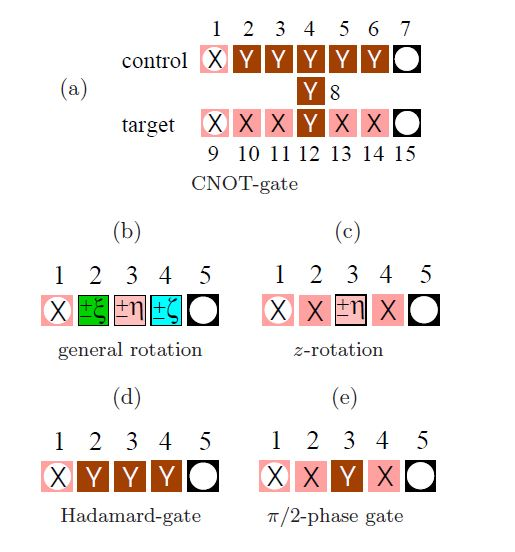
\includegraphics[scale=0.8]{gfx/gates.JPG}
\caption{Universal set of quantum gates \citep{raussendorf_measurement-based_2003}}
\label{fig:universal_set}
\end{figure}